\section{Pianificazione}
I diagrammi delle attività presenti in questa sezione sono stati rappresentati 
tramite l'uso di diagrammi di Gantt.

\subsection{Analisi dei Requisiti}
\textbf{Periodo:} 04/03/2016 - 31/03/2016\\
Questa fase prevedere la scelta e l'implementazione degli strumenti necessari 
per definire il \textit{repository}\G\ utilizzato dal \textit{team}\G, le 
norme di base per sviluppare una documentazione quanto più possibile omogenea e 
coerente, una pianificazione che guida lo sviluppo del progetto. Termina con 
la scadenza di consegna dell'offerta, cioè con la consegna della 
\textit{Revisione dei Requisiti}.\\\\
I ruoli attivi in questa fase sono:

\begin{itemize}
	\item Responsabile;
	\item Amministratore;
	\item Analista;
	\item Progettista;
	\item Verificatore.
\end{itemize}
Le attività da svolgersi in questa fase sono:
\begin{itemize}
	\item \textbf{Ricerca ed implementazione degli strumenti}: 
	l'\textit{Amministratore di Progetto} ha il compito di scegliere, 
	implementare e configurare gli strumenti necessari al lavoro del team. Deve 
	apprendere il funzionamento e fare formazione ai rimanenti membri del 
	\textit{team\G} di sviluppo;
	\item \textbf{Norme di Progetto}: attività svolta 
	dall'\textit{Amministratore di 
	Progetto}. Concordati con il \textit{team}\G\ gli strumenti da utilizzare, 
	si procede 	alla stesura di un serie di norme, che dovranno essere 
	rispettate dai membri del team per tutta la durata del progetto. Le norme 
	sono interne al \textit{team}\G\ e non legate al capitolato SiVoDiM;
	\item \textbf{Studio di fattibilità}: è compito degli \textit{Analisti} 
	valutare ogni capitolato e redarre uno Studio di fattibilità, dal quale si 
	delinea chiaramente quale capitolato è stato scelto e la motivazione che ha 
	guidato a tale scelta.
	\item \textbf{Piano di Progetto}: qui vengono pianificate le attività, 
	risorse e costi della gestione del \textit{team}\G. Poi riportate in modo 
	strutturato nel \textit{Piano di Progetto v1.0.0};
	\item \textbf{Analisi dei Requisiti}: gli \textit{Analisti} hanno 
	l'incarico di ricercare i requisiti e di redigere il documento 
	\textit{Analisi dei Requisiti v1.0.0}, con Diagrammi dei Casi D'Uso (UC\G). 
	Questa attività è poco legata	al proponente\G, data la natura vaga del 
	Capitolato\G\ fornito dall'azienda MIVOQ s.r.l.;
	\item \textbf{Piano di Qualifica}: descrizione su strategie di verifica e 
	validazione adottate. Documentate poi nel \textit{Piano di Progetto v1.0.0};
	\item \textbf{Glossario}: attività parallela alla stesura di tutti i 
	documenti sopracitati. Il \textit{Glossario v1.0.0} verrà aggiornato in 
	modo incrementale fino al completamento della documentazione;
	\item \textbf{Verbale incontri}: per analizzare i requisiti presentati nel 
	Capitolato \G\ vengono organizzati incontri, in seguito documentati con 
	verbali formali.
\end{itemize}

\newpage
\begin{figure}
	\centering
	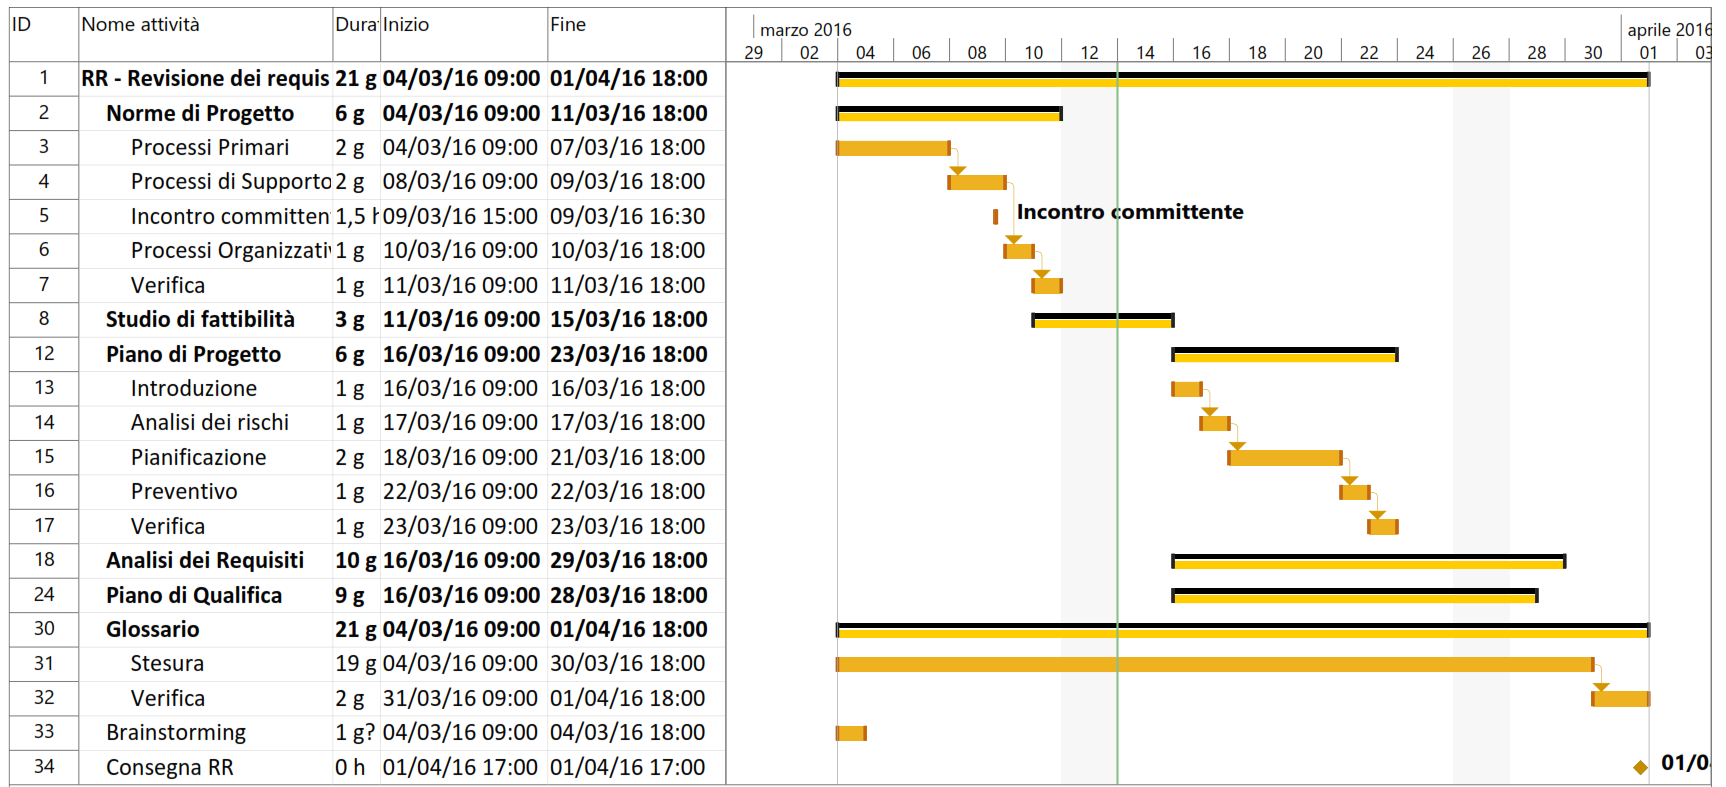
\includegraphics[width= 16cm]{AR.png}
	\caption{Analisi dei Requisiti}
\end{figure}


\subsection{Analisi di Dettaglio}
\textbf{Periodo:} 01/04/2016 - 18/04/2016\\
Questa attività ha termine con la presentazione in data 18/04/2016 dell'Analisi 
dei Requisiti\\\\
I ruoli attivi in questa fase sono:

\begin{itemize}
	\item Responsabile;
	\item Amministratore;
	\item Analista;
	\item Progettista;
	\item Verificatore.
\end{itemize}
Questa fase ha lo scopo di integrare e consolidare i requisiti ottenuti 
precedentemente.

\newpage
\begin{figure}
	\centering
	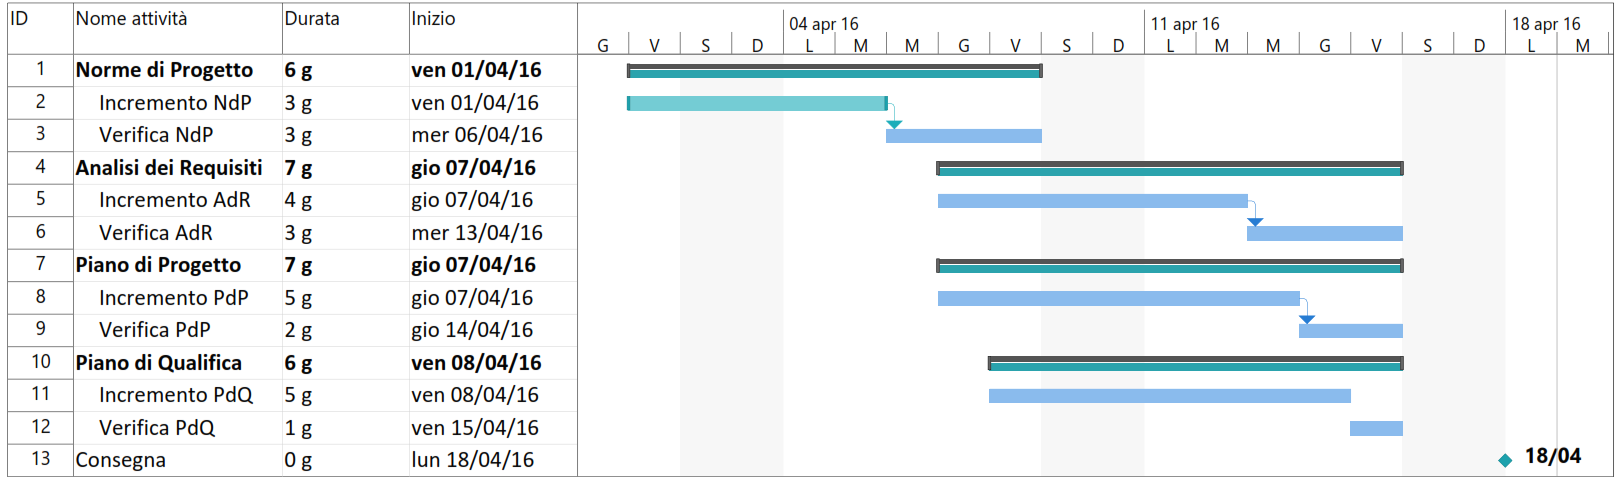
\includegraphics[width= 16cm]{AD.png}
	\caption{Analisi di Dettaglio}
\end{figure}

\subsection{Progettazione Architetturale}
\textbf{Periodo:} 19/04/2016 - 23/05/2016\\

\subsection{Progettazione di Dettaglio e Codifica}
\textbf{Periodo:} 24/05/2016 - 17/06/2016\\

\subsection{Validazione}
\textbf{Periodo:} 18/06/2016 - 11/07/2016\\